\documentclass[12pt]{extarticle}
\usepackage[utf8]{inputenc}
\usepackage[toc,page]{appendix}
\usepackage[maxbibnames=99,backend=bibtex]{biblatex}
\usepackage{listings}
\usepackage{float}
\usepackage[left=3.5cm,right=2.5cm]{geometry}
\usepackage{hyperref}
\usepackage{graphicx}
\graphicspath{ {./res/} }
\usepackage{listings}
\usepackage{color} %red, green, blue, yellow, cyan, magenta, black,white
\definecolor{mygreen}{RGB}{28,172,0} % color values Red, Green, Blue
\definecolor{mylilas}{RGB}{170,55,241}

\lstset{language=Matlab,%
    %basicstyle=\color{red},
    breaklines=true,%
    morekeywords={matlab2tikz},
    keywordstyle=\color{blue},%
    morekeywords=[2]{1}, keywordstyle=[2]{\color{black}},
    identifierstyle=\color{black},%
    stringstyle=\color{mylilas},
    commentstyle=\color{mygreen},%
    showstringspaces=false,%without this there will be a symbol in the places where there is a space
    numbers=left,%
    numberstyle={\tiny \color{black}},% size of the numbers
    numbersep=9pt, % this defines how far the numbers are from the text
    emph=[1]{for,end,break},emphstyle=[1]\color{red}, %some words to emphasise
    %emph=[2]{word1,word2}, emphstyle=[2]{style},    
}

\renewcommand{\contentsname}{Index}
\begin{document}

\begin{titlepage}

    \begin{figure}
      \centering
      
\includegraphics[scale=0.3]{images/cherubino.jpeg}
    \end{figure}

    \begin{center}
      MSc in Computer Engineering\\
      Electronic systems\\
      \vspace*{5\baselineskip}
      \textbf{\large FIR low pass filter}\\
      Project discussion and VHDL implementation
    \end{center}
    \vspace*{7\baselineskip}
    \null\hfill Gioele Carignani

    \begin{center}
        2017/2018
    \end{center}
\end{titlepage}
\tableofcontents{}
\clearpage
\clearpage
\section{Introduction}
In signal processing, a finite impulse response (FIR) filter is a filter whose impulse response, or response to any other finite length input, is of finite duration, because it settles to zero in finite time. 
The impulse response of an Nth-order discrete-time FIR filter lasts exactly N + 1 samples (from first nonzero element through last nonzero element) before it then settles to zero.
For a causal discrete-time FIR filter of order N, each value of the output sequence is a weighted sum of the most recent input values:
\begin{center}
$$ y[n]=\sum_{i=0}^{N}c{_{i}}\cdot x[n-i]$$
\end{center}
\subsection{Filter Design}
When a particular frequency response is desired, several different design methods are possible, for example:
\begin{itemize}
  \item {Window design method:} we first design an ideal IIR filter and then truncate the result by multiplying it with a finite length window function.
  \item {Frequency Sampling method:} this technique is the most direct technique imaginable when a desired frequency response has been specified. It consists simply of uniformly sampling the desired frequency response, and performing an inverse DFT to obtain the corresponding (finite) impulse response.
  \item {Parks-McClellan method:} The Remez exchange algorithm is commonly used to find an optimal equiripple set of coefficients. Here the user specifies a desired frequency response, a weighting function for errors from this response, and a filter order N. The algorithm then finds the set of N+1 coefficients that minimize the maximum deviation from the ideal. 
\end{itemize}
\subsection{Applications}Finite-impulse response (FIR) digital filter is widely used in several digital signal processing applications, such as speech processing, loud speaker equalization, echo cancellation, adaptive noise cancellation, and various communication applications, including software-defined radio (SDR) and so on. Many of these applications require FIR filters of large order to meet the stringent frequency specifications. Very often these filters need to support high sampling rate for high-speed digital communication. The number of multiplications and additions required for each filter output, however, increases linearly with the filter order. 

\section{Architectures}
Different type of architectures are available depending on the speed and power constraints.
To fulfill desired specifications the following optimizations can be done:\\
\begin{itemize}
    \item Reduce total number of operations, in particular multiplications that are heavier
    \item Fixed-point arithmetic is cheaper and faster
    \item The area of a fixed point parallel multiplier is proportional to the product of the coefficient and data word lengths one could try to reduce their word length
\end{itemize}
Suppose a filter of order N has to be realized.
\subsection{Direct form}
This structure requires N memory locations for storing previous inputs and in terms of complexity it does N+1 multiplications and  N additions.  For building this structure the definition of Equation \ref{eq:general} is used to derive the equivalent circuit.
\begin{figure}[H]
    \centering
    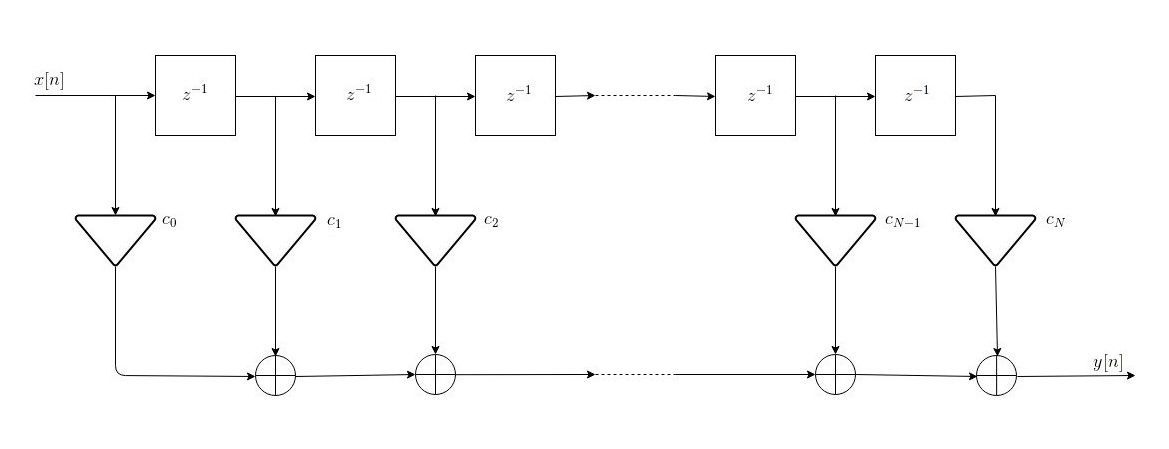
\includegraphics[scale=0.45]{images/direct.jpeg}    
    \caption{scheme of direct form}
    \label{fig:my_label}
\end{figure}
\subsection{Transposed form}
This structure is very similar at first look w.r.t. the previous one but in the former there was a big addition in the end, here instead there is a set of small additions separated by delay elements.
\begin{figure}[H]
    \centering
    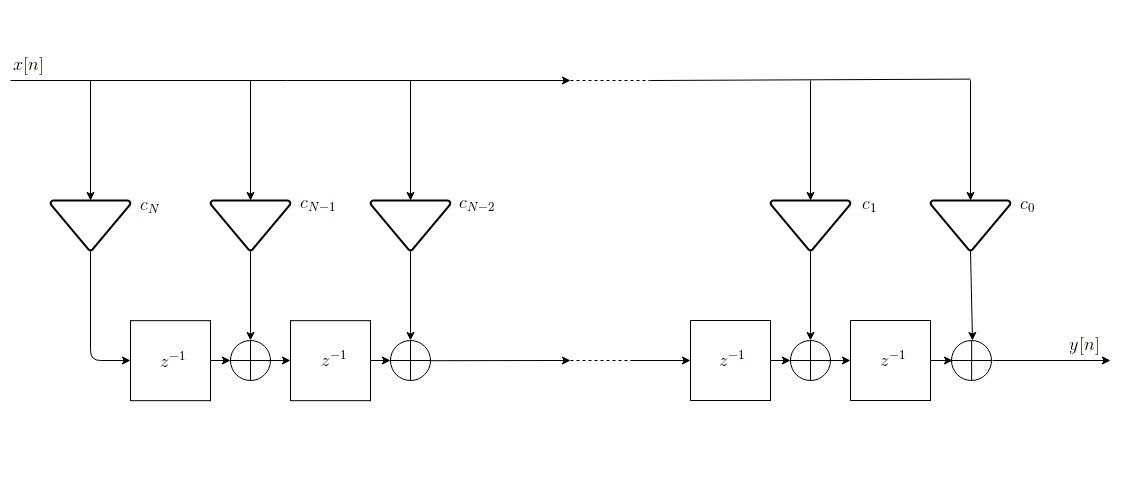
\includegraphics[scale=0.45]{images/transposed.jpg}    
    \caption{scheme of transposed form}
    \label{fig:transposed}
\end{figure}
\subsection{Symmetric taps (linear phase)}
FIR filters are often designed to have symmetry in the filter taps so exploit this symmetry can be exploited in order to reduce the number of multiplications.
$$y[n]= c_{0}(x[n]+x[0])+c_{1}(x[n-1]+x[1])+....+c_{N/2}(x[N/2])$$
The last term of the previous equation is needed only if N is even.
With this type of implementation the number of multiplications is reduced to $\left \lfloor N/2+1 \right \rfloor$
\begin{figure}[H]
    \centering
    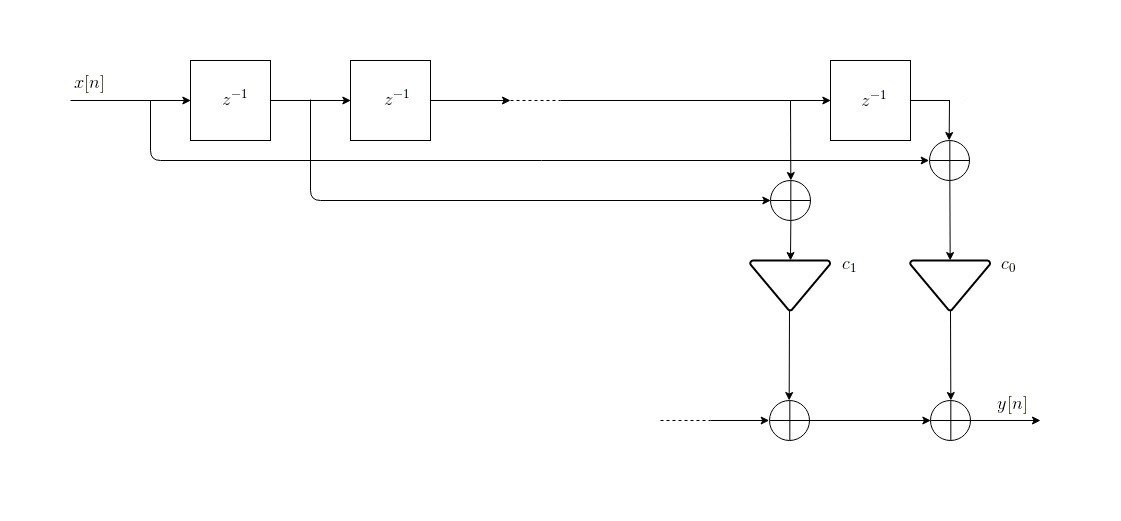
\includegraphics[scale=0.45]{images/symmetryc.jpg}    
    \caption{direct form with symmetric taps}
    \label{fig:symmetric}
\end{figure}
\subsection{Cascade form}
The transfer function is expressed as product of second-order polynomial system functions via factorization:
\begin{equation} \label{eq:1}
H(z)=\frac{y[n]}{x[n]} =\sum_{i=0}^{N}c_{i}z^{-i}= \prod_{i=1}^{M_{c}}(\beta_{0i}+\beta_{1i}z^{-1}+\beta_{2i}z^{-2})
\end{equation}
Where $M_{c}= \left \lfloor (N+1)/2 \right \rfloor$.
Assuming that N is even, this implementation needs N storage elements, $\frac{3N}{2}$ multiplications and N additions for each output value.
\begin{figure}[H]
    \centering
    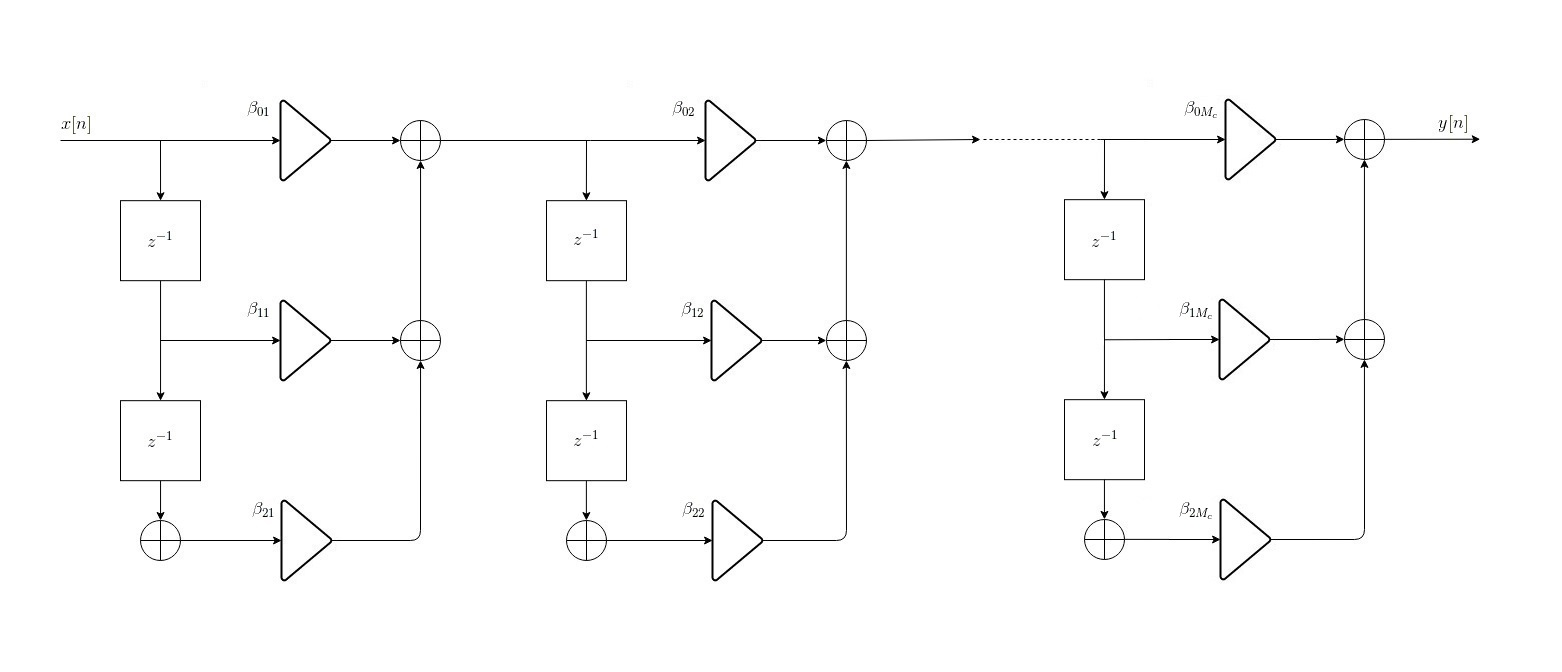
\includegraphics[scale=0.35]{images/cascade.jpg}    
    \caption{cascade form}
    \label{fig:cascade}
\end{figure}
To save computational complexity, Equation (\ref{eq:1}) is expressed as:
\begin{equation} \label{eq:2}
H(z)= G\prod_{i=1}^{M_{c}}(1+\beta_{1i}'z^{-1}+\beta_{2i}'z^{-2})
\end{equation}
where $G=\beta_{01}\beta_{02} \cdot\cdot\cdot\beta_{0M_{c}}$ ,$\beta_{1i}'=\beta_{1i}/\beta_{0i}$ , $i= 1,2,\cdot \cdot \cdot,M_{c}$ in this way all $\beta_{0i}$ are normalized to 1 as one can see in (Equation \ref{eq:2}). Assuming that N is even N delay elements are needed, (N+1) multiplications and N additions, for computing each output value.
\begin{figure}[H]
    \centering
    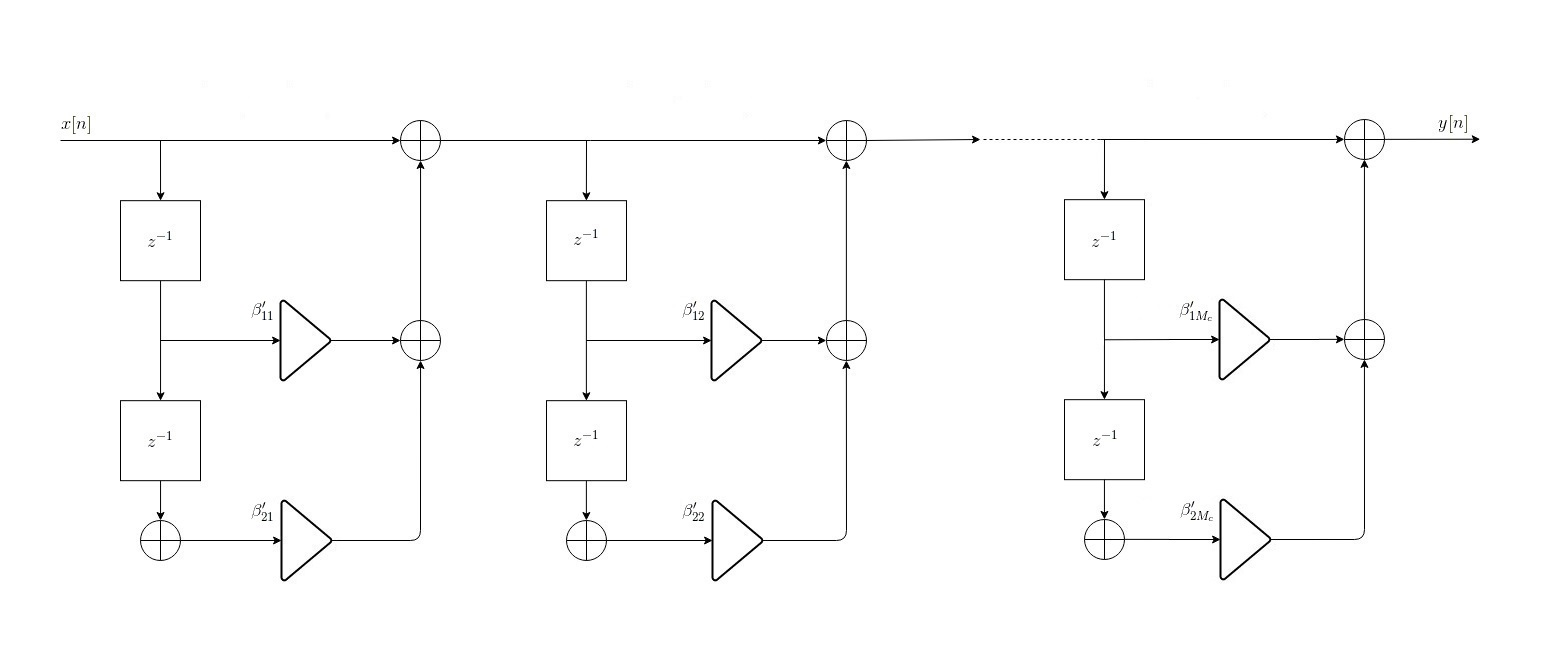
\includegraphics[scale=0.35]{images/cascadeoptimised.jpg}    
    \caption{cascade form with lower complexity}
    \label{fig:cascade_opt}
\end{figure}

\section{Implemented Architecture}
After analyzing the different architectures the transposed form was implemented due to its overall realization simplicity and it is the architecture that has the shortest path registry-logic-registry hence it permits to reduce the timing on the critical path and increase the clock frequency reachable when the VHDL code will be mapped on FPGA. A drawback w.r.t. the direct form is that this solution brings a higher latency for the input data that will have to traverse the entire registry chain, nevertheless once the nework is at regime it will output new data per each clock cycle.
\section{Integer conversion}
The coefficients that are doubles had to be converted to integer on 16 bits through the following script:
\lstinputlisting{../Matlab/coeff_script.m}
\subsection{Output size}
\label{sec:sizing}
To realize the transposed architecture the result had to be sized:
\begin{equation}
	\left \lceil log_2(2^{b-1})*\sum_{i=0}^{N} coeff_i\right \rceil	
	\label{eq:size}
\end{equation}
Equation \ref{eq:size} returned a value for the output dimension of 31 bits.
\section{Test Plan}
In order to test the effectiveness of the filter the mathematical limits given by the size of the input and on the coefficient values had to be tested.
To ease the testing of the filter with different inputs the test bench reads/writes data from/to file.
\subsection{Size limits}
To stress out the size limits computed in section \ref{sec:sizing} the filter has been feeded with maximum value in modulus i.e. ($-2^(b-1)= -32768 $) repeated continuosly and checked if the output corresponded to the value given by applying in Matlab expression \ref{eq:general}, the results can be seen in the following figure:
\begin{figure}[H]
  \centering
  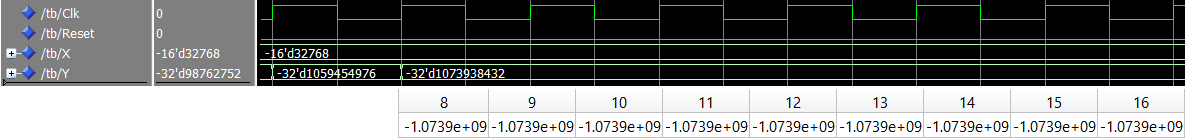
\includegraphics[width=0.9\linewidth]{./images/simul32768.PNG}
  \caption{We can see how at regime the network output corresponds to the value returned by matlab}
  \label{fig:32768}
\end{figure}
\section{Synthesis} % (fold)
For the hardware implementation of the project Vivado software by Xilinx was used. This software enabled to map the VHDL code on Zynq-7000 board. To reach the final implementation and discover the maximum operating frequency the typical flow of Vivado was followed i.e. from VHDL code to RTL analysis, synthesis and as last implementation.
\label{sec:synthesis_and_implementation}
\subsection{RTL Design}
\begin{figure}[H]
  \centering
  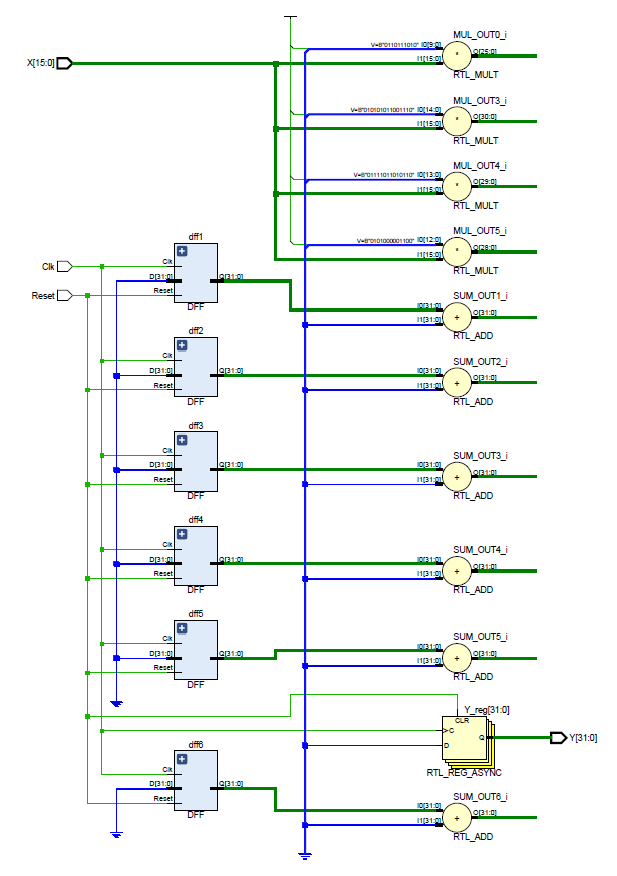
\includegraphics[width=0.5\linewidth]{./images/schematic.PNG}
  \caption{RTL design from vivado}
  \label{fig:schematic}
\end{figure}
\subsection{Synthesis}
A clock period of 10 ns was set. The synthesis was carried without any kind of warnings displayed.\\

\subsubsection{Timing report} % (fold)
\label{ssub:timing_report}
Timing report is fine and states that all constraints are met:
\begin{figure}[H]
  \centering
  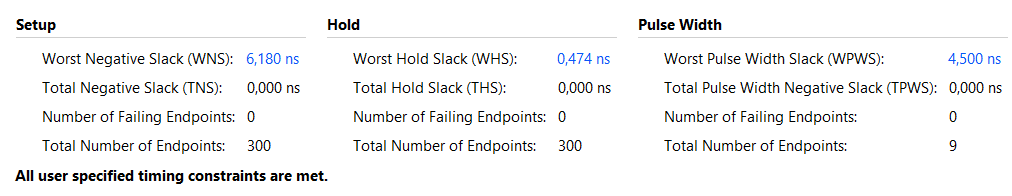
\includegraphics[width=0.9\linewidth]{./images/timing.PNG}
  \caption{Timing summary from vivado}
  \label{fig:timing}
\end{figure}


\subsubsection{Power report} % (fold)
\label{ssub:power_report}
\begin{figure}[H]
  \centering
  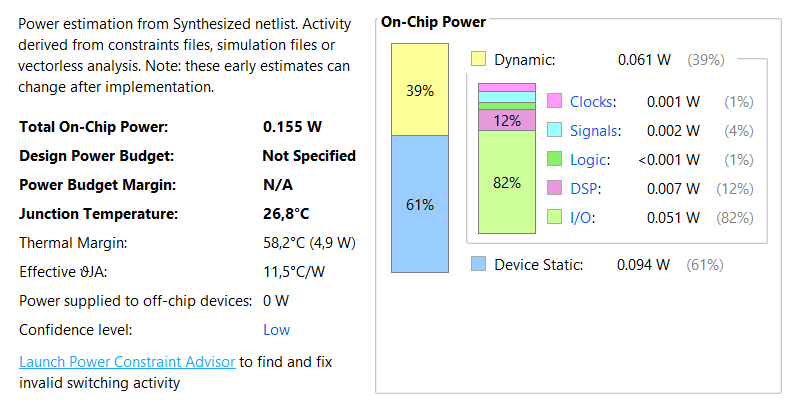
\includegraphics[width=0.9\linewidth]{./images/power.PNG}
  \caption{Power summary from vivado}
  \label{fig:power}
\end{figure}

\subsubsection{Utilization report} % (fold)
\label{ssub:utilization_report}
\begin{figure}[H]
  \centering
  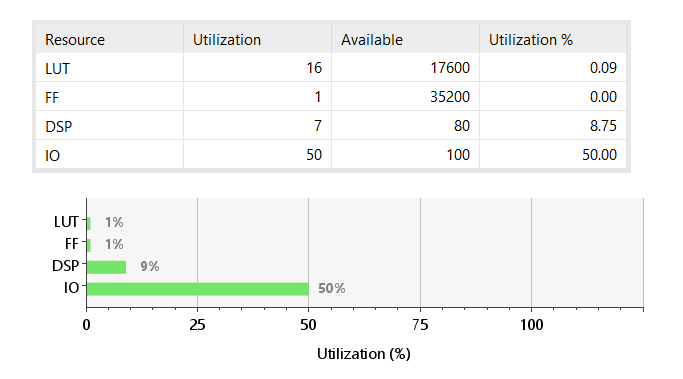
\includegraphics[width=0.9\linewidth]{./images/utilization.PNG}
  \caption{Utilization summary from vivado}
  \label{fig:utilization}
\end{figure}
Figure \ref{fig:utilization} shows how the most widely used resource is the I/O this derives from the fact that the circuit has 16 bit inputs and a 32 bit output.
\subsection{Critical path} % (fold)
\label{sub:critical_path}
Vivado shows how the critical path includes the sum and multiplication operation from the output of a registry till the input to the next registry.
 \begin{figure}[H]
   \centering
   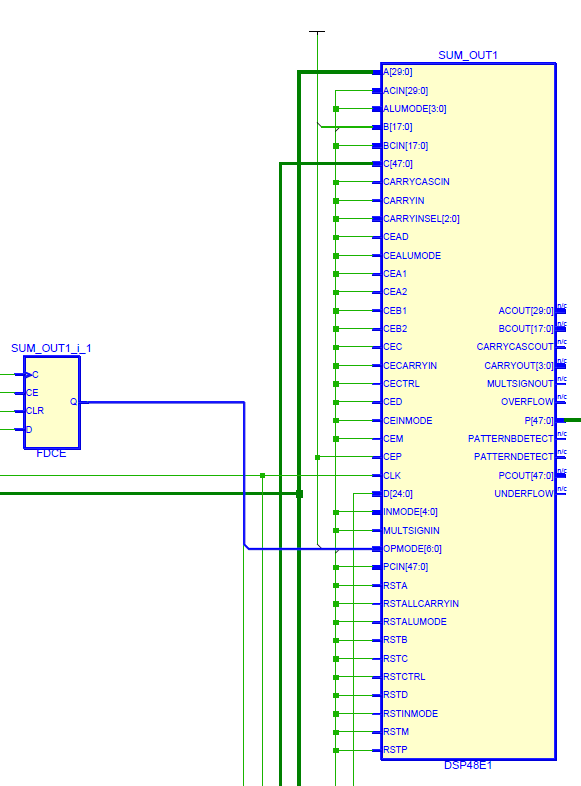
\includegraphics[width=0.5\linewidth]{./images/critical}
   \caption{Critical path highlighted by vivado}
   \label{fig:critical}
 \end{figure}
\subsection{Maximum operating frequency} % (fold)
\label{sub:maximum_operating_frequency}
From the timing report a positive Worst Negative Slack suggests that the circuit is not operating at the maximum frequency possible.
\begin{equation}
	f_{max} = \frac{1}{t_{clk}-slack}=\frac{1}{10ns-6.18ns}= \frac{1}{3.82ns}= 260 Mhz
	\label{eq:fmax}
\end{equation}
Equation \ref{eq:fmax} states that the maximum frequency at which the clock can be guided is 260 Mhz.

\section{Implementation}
The implementation was carried out without any warning. The data reported by the implementation confirm the conclusion derived in the synthesis step with slight differences such as the fact that the worst negative slack is now of $6.017ns$ hence the circuit has a maximum operating frequency of $251.1Mhz$ due to I/O ports being actually assigned and this brings some delay. 

\section{Conclusions}
The work can be considered concluded, since the filter is compliant to its specifications. To reduce the number of multiplications the symmetric version of the filter could be developed since symmetric coefficients are given. The filter precision could be improved by increasing the number of coefficients hence the number of steps obtaining a behavior more similar to an ideal filter. 
\end{document}
